
\section{Redes Recurrentes}

\begin{frame}
	\frametitle{Red Recurrente (RNN): Una RNA con memoria}

	\begin{center}
		\begin{tikzpicture}[node distance=1.5cm, auto]
			% Estilos de nodos
			\tikzstyle{neuron} = [rectangle, rounded corners, minimum width=1.5cm, minimum height=0.75cm,text centered, draw=black, fill=red!30]
			\tikzstyle{arrow} = [thick,->,>=stealth]
			
			% Nodos RNN
			\node[neuron] (rnn1) {RNN};
			\node[neuron, right=of rnn1] (rnn2) {RNN};
			\node[neuron, right=of rnn2] (rnn3) {RNN};
			
			% Nodos de estados h
			\node[left=of rnn1] (h0) {$h_{t-2}$};
			\node[right=of rnn3] (h3) {$h_{t+1}$};
			
			% Flechas para h
			\draw [arrow] (h0) -- (rnn1);
			\draw [arrow] (rnn1) -- node[above] {$h_{t-1}$} (rnn2);
			\draw [arrow] (rnn2) -- node[above] {$h_t$} (rnn3);
			\draw [arrow] (rnn3) -- (h3);
			
			% Nodos de entrada x y flechas
			\node[below=of rnn1] (x1) {$\vec{x}_{t-1}$};
			\node[below=of rnn2] (x2) {$\vec{x}_t$};
			\node[below=of rnn3] (x3) {$\vec{x}_{t+1}$};
			\draw [arrow] (x1) -- (rnn1);
			\draw [arrow] (x2) -- (rnn2);
			\draw [arrow] (x3) -- (rnn3);
			
			% Nodos de salida y y flechas
			\node[above=of rnn1] (y1) {$\hat{y}_{t-1}$};
			\node[above=of rnn2] (y2) {$\hat{y}_t$};
			\node[above=of rnn3] (y3) {$\hat{y}_{t+1}$};
			\draw [arrow] (rnn1) -- (y1);
			\draw [arrow] (rnn2) -- (y2);
			\draw [arrow] (rnn3) -- (y3);
		\end{tikzpicture}
	\end{center}

\end{frame}

\begin{frame}
	\frametitle{Observaciones sobre las RNN}
	\begin{itemize}
		\item Cada 'rectángulo' RNN representa exactamente la misma Red Neuronal (con los mismos parámetros, capas, neuronas, tasa de aprendizaje) \textit{solo que en diferentes tiempos}.
		
		\item Cada salida $\hat{y}_{ti}$ es la predicción que el modelo arroja en un tiempo $ti$
		
		\item Cada salida que retroalimenta a la misma red $h_{ti}$ se conoce como \textit{estado oculto} y representa la memoria a corto plazo de la Red Neuronal, pues enviá información de la activación de la misma red pero del estado anterior.
		
	\end{itemize}
\end{frame}

\begin{frame}
	\frametitle{Representación de una RNN}
	
	
	\begin{columns}
		\begin{column}{0.48\textwidth}
			\begin{center}
				\begin{tikzpicture}[node distance=1cm and 0.5cm, auto, scale=0.8, transform shape]
					% Estilos de nodos
					\tikzset{
						rect/.style={rectangle, rounded corners, minimum width=2.5cm, minimum height=1cm, text centered, draw=black, fill=red!30},
						arrow/.style={thick,->,>=stealth}
					}
					
					% Nodos
					\node[rect] (rnn) {RNN};
					\node[below=of rnn] (x) {$x_t$};
					\node[left=of rnn] (hprev) {$h_{t-1}$};
					\node[right=of rnn] (hnext) {$h_t$};
					\node[above=of rnn] (y) {$y_t$};
					
					% Flechas
					\draw[arrow] (x) -- (rnn);
					\draw[arrow] (rnn) -- (y);
					\draw[arrow] (hprev) -- (rnn);
					\draw[arrow] (rnn) -- (hnext);
					
					% Loop para h
					\draw[arrow] (hnext.east) -- ++(0.5,0) -- ++(0, -3) -| (hprev.south);
				\end{tikzpicture}
			\end{center}
		\end{column}
		\begin{column}{0.48\textwidth}
			\begin{center}
				Al observar el diagrama anterior se suele pensar que se cuenta con una Red Neuronal \textit{diferente} para cada tiempo $t$, por ello es mejor usar su representación con lazo de retroalimentación.
			\end{center}
		\end{column}
	\end{columns}
	
	
\end{frame}

%------------------------------------------------

\begin{frame}
	\frametitle{RNN y las Secuencias}
	\vspace{-2mm}
	Angelito va en el metro camino a su casa y se encuentra en esta estación... \textit{¿Cuál es la siguiente?}
	\vspace{8mm}
	
	\begin{tikzpicture}[node distance=2cm and 0cm]
		% Dibujo del cuadro alrededor de la red neuronal con color de fondo crema y esquinas redondeadas
		% Ajustar el rectángulo para que sea más estrecho y no tan ancho
		\fill[cream, rounded corners] (3,0.5) rectangle (8,4.5); % Se ajusta para ser más estrecho
		
		% Capa de entrada, centrada dentro del cuadro crema
		\foreach \y in {1,2,3,4}
		\node[circle, draw, fill=blue!50] (Input-\y) at (4,\y) {};
		
		% Capa oculta, centrada dentro del cuadro crema
		\foreach \y [count=\s] in {1.5,2.5,3.5}
		\node[circle, draw, fill=green!50] (Hidden-\s) at (5.5,\y) {};
		
		% Capa de salida, centrada dentro del cuadro crema
		\node[circle, draw, fill=red!50] (Output) at (7,2.5) {};
		
		% Conexiones
		\foreach \y in {1,2,3,4}
		\foreach \s in {1,...,3}
		\draw[->] (Input-\y) -- (Hidden-\s);
		\foreach \s in {1,...,3}
		\draw[->] (Hidden-\s) -- (Output);
		
		% Imagen de entrada, centrada con respecto a la red neuronal
		\node[anchor=center] (image) at (1cm,2.5cm) {
\includegraphics[width=.2\textwidth]{pinosuarez.png}};
		
		
		% Flecha desde la imagen de entrada a las neuronas de entrada
		\draw[->] (image.east) -- ($(Input-2)!.5!(Input-3)$);
		
		% Imagen de predicción, movida más hacia la derecha
		\node[right=3cm of Output.center, anchor=center] (prediccion) {
\includegraphics[width=.25\textwidth]{merced.png}};
		
		% Flecha desde la capa de salida a la imagen de predicción
		\draw[->] (Output) -- (prediccion.west);
	\end{tikzpicture}
	
\end{frame}


\begin{frame}
	\frametitle{RNN y las Secuencias}
	Ahora, \textit{como todos los días}... Angelito llega al metro Pantitlán... ¿Qué estación sigue?
	
	\begin{tikzpicture}[node distance=2cm and 0cm]
		% Dibujo del cuadro alrededor de la red neuronal con color de fondo crema y esquinas redondeadas
		% Ajustar el rectángulo para que sea más estrecho y no tan ancho
		\fill[cream, rounded corners] (3,0.5) rectangle (8,4.5); % Se ajusta para ser más estrecho
		
		% Capa de entrada, centrada dentro del cuadro crema
		\foreach \y in {1,2,3,4}
		\node[circle, draw, fill=blue!50] (Input-\y) at (4,\y) {};
		
		% Capa oculta, centrada dentro del cuadro crema
		\foreach \y [count=\s] in {1.5,2.5,3.5}
		\node[circle, draw, fill=green!50] (Hidden-\s) at (5.5,\y) {};
		
		% Capa de salida, centrada dentro del cuadro crema
		\node[circle, draw, fill=red!50] (Output) at (7,2.5) {};
		
		% Conexiones
		\foreach \y in {1,2,3,4}
		\foreach \s in {1,...,3}
		\draw[->] (Input-\y) -- (Hidden-\s);
		\foreach \s in {1,...,3}
		\draw[->] (Hidden-\s) -- (Output);
		
		% Imagen de entrada, centrada con respecto a la red neuronal
		\node[anchor=center] (image) at (1cm,2.5cm) {
\includegraphics[width=.2\textwidth]{panti.png}};
		
		
		% Flecha desde la imagen de entrada a las neuronas de entrada
		\draw[->] (image.east) -- ($(Input-2)!.5!(Input-3)$);
		
		% Imagen de predicción, movida más hacia la derecha
		\node[right=3cm of Output.center, anchor=center] (prediccion) {
\includegraphics[width=.25\textwidth]{pregunta.jpg}};
		
		% Flecha desde la capa de salida a la imagen de predicción
		\draw[->] (Output) -- (prediccion.west);
	\end{tikzpicture}
	
\end{frame}



\begin{frame}
	\frametitle{Problema: \textbf{Memoria a corto plazo}}
	Ahora, \textit{como todos los días}... Angelito llega al metro Pantitlán... ¿Qué estación sigue?
	
	\begin{tikzpicture}[node distance=2cm and 0cm]
		% Dibujo del cuadro alrededor de la red neuronal con color de fondo crema y esquinas redondeadas
		% Ajustar el rectángulo para que sea más estrecho y no tan ancho
		\fill[cream, rounded corners] (3,0.5) rectangle (8,4.5); % Se ajusta para ser más estrecho
		
		% Capa de entrada, centrada dentro del cuadro crema
		\foreach \y in {1,2,3,4}
		\node[circle, draw, fill=blue!50] (Input-\y) at (4,\y) {};
		
		% Capa oculta, centrada dentro del cuadro crema
		\foreach \y [count=\s] in {1.5,2.5,3.5}
		\node[circle, draw, fill=green!50] (Hidden-\s) at (5.5,\y) {};
		
		% Capa de salida, centrada dentro del cuadro crema
		\node[circle, draw, fill=red!50] (Output) at (7,2.5) {};
		
		% Conexiones
		\foreach \y in {1,2,3,4}
		\foreach \s in {1,...,3}
		\draw[->] (Input-\y) -- (Hidden-\s);
		\foreach \s in {1,...,3}
		\draw[->] (Hidden-\s) -- (Output);
		
		% Imagen de entrada, centrada con respecto a la red neuronal
		\node[anchor=center] (image) at (1cm,2.5cm) {
\includegraphics[width=.2\textwidth]{panti.png}};
		
		
		% Flecha desde la imagen de entrada a las neuronas de entrada
		\draw[->] (image.east) -- ($(Input-2)!.5!(Input-3)$);
		
		% Imagen de predicción, movida más hacia la derecha
		\node[right=3cm of Output.center, anchor=center] (prediccion) {
\includegraphics[width=.25\textwidth]{esponja.jpeg}};
		
		% Flecha desde la capa de salida a la imagen de predicción
		\draw[->] (Output) -- (prediccion.west);
	\end{tikzpicture}
\end{frame}

\begin{frame}
	\frametitle{Problema: \textbf{Memoria a corto plazo}}
	
	\begin{columns}
		\begin{column}{0.5\textwidth}
			\begin{itemize}
				\item Prácticamente, la Red Neuronal Recurrente solo obtiene información del \textit{estado inmediato anterior}.
				\item No se acuerda de lo que paso en tiempos muy alejados al presente.
				\item No puede hacer predicciones certeras a futuro
			\end{itemize}
		\end{column}
		\begin{column}{0.5\textwidth}
			\begin{center}
				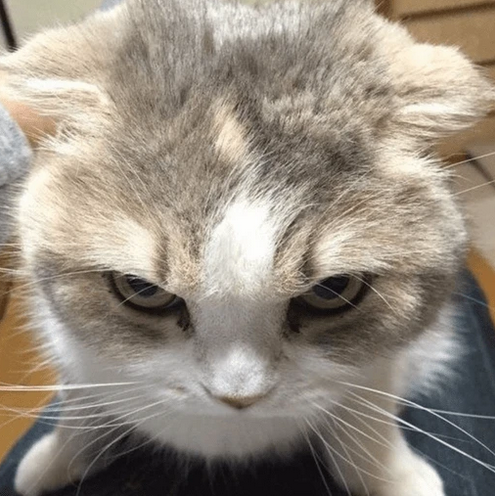
\includegraphics[width=0.9\linewidth]{enojado.png}
			\end{center}
		\end{column}
	\end{columns}
\end{frame}


\begin{frame}
	\frametitle{Problema: \textbf{Memoria a corto plazo}}
	
	\begin{columns}
		\begin{column}{0.5\textwidth}
			\begin{center}
				
\includegraphics[width=0.9\linewidth]{gp.png}
			\end{center}
		\end{column}
		\begin{column}{0.5\textwidth}
			\begin{center}
				¿La solución?
				
				\textbf{LA CELDA LSTM}
				
				\textit{(Long Short-Term Memory)}
			\end{center}
		\end{column}
	\end{columns}
\end{frame}

%------------------------------------------------

